\documentclass[hyperref,adobefonts]{ctexart}

\providecommand{\tightlist}{\setlength{\itemsep}{0pt}\setlength{\parskip}{0pt}}

\usepackage{lmodern}
\usepackage{amssymb,amsmath}
\usepackage{ifxetex,ifluatex}
\usepackage{fixltx2e} % provides \textsubscript
\ifnum 0\ifxetex 1\fi\ifluatex 1\fi=0 % if pdftex
  \usepackage[T1]{fontenc}
  \usepackage[utf8]{inputenc}
\else % if luatex or xelatex
  \ifxetex
    \usepackage{xltxtra,xunicode}
  \else
    \usepackage{fontspec}
  \fi
  \defaultfontfeatures{Mapping=tex-text,Scale=MatchLowercase}
  \newcommand{\euro}{€}
\fi
% use upquote if available, for straight quotes in verbatim environments
\IfFileExists{upquote.sty}{\usepackage{upquote}}{}
% use microtype if available
\IfFileExists{microtype.sty}{%
\usepackage{microtype}
\UseMicrotypeSet[protrusion]{basicmath} % disable protrusion for tt fonts
}{}
\usepackage[tmargin=2.5cm, bmargin=1.5cm, rmargin=2.5cm, lmargin=2.5cm]{geometry}

\usepackage{longtable,booktabs}

\usepackage{graphicx}
\makeatletter
\def\maxwidth{\ifdim\Gin@nat@width>\linewidth\linewidth\else\Gin@nat@width\fi}
\def\maxheight{\ifdim\Gin@nat@height>\textheight\textheight\else\Gin@nat@height\fi}
\makeatother
% Scale images if necessary, so that they will not overflow the page
% margins by default, and it is still possible to overwrite the defaults
% using explicit options in \includegraphics[width, height, ...]{}
\setkeys{Gin}{width=\maxwidth,height=\maxheight,keepaspectratio}
\setlength{\parindent}{0pt}
\setlength{\parskip}{6pt plus 2pt minus 1pt}
\setlength{\emergencystretch}{3em}  % prevent overfull lines
\setcounter{secnumdepth}{5}

\title{天津医科大学试卷分析}
\author{伊现富}
\date{2018-07-12}
\hypersetup{colorlinks,linkcolor=black}

\begin{document}
\maketitle

{
\setcounter{tocdepth}{2}
\tableofcontents
}
\section{试卷基本信息}

课程名称:Linux系统概论;授课教师:伊现富;开课院系:生物医学工程与技术学院;学分:2;学时:36;考生专业:生物信息学;考生年级:2016级;考生人数:28;试卷类型:A卷(闭卷);试卷总分:100;考试时间:2018-07-12。

\section{整卷质量分析}

\subsection{统计数据}

\begin{longtable}{c|c|c|c|c|c|c|c|c}
\hline
student & item & grade & mean & sd & var & median & mode & pass\\
\hline
28 & 72 & 100 & 71.14 & 15.83 & 250.57 & 73.5 & 69,89 & 82.14\\
\hline
\end{longtable}

\begin{longtable}{c|c|c|c|c|c|c|c}
\hline
max & min & range & skewness & kurtosis & mean(H) & mean(M) & mean(L)\\
\hline
94 & 26 & 68 & -0.96 & 3.9 & 87.62 & 73 & 51.88\\
\hline
\end{longtable}

\begin{itemize}
\tightlist
\item
  偏度(skewness):衡量实数随机变量概率分布的不对称性,偏度的绝对值数值越大表示其分布形态的偏斜程度越大。偏度为0表示数值相对均匀地分布在平均值的两侧(但不一定意味着其为对称分布);偏度大于0为正偏态或右偏态(右侧的尾部更长,分布的主体集中在左侧);偏度小于0为负偏态或左偏态(左侧的尾部更长,分布的主体集中在右侧)。
\item
  峰度(kurtosis):衡量实数随机变量概率分布的峰态,峰度的绝对值数值越大表示其分布形态的陡缓程度与正态分布的差异程度越大。峰度为0表示总体数据分布与正态分布的陡缓程度相同;峰度大于0表示总体数据分布与正态分布相比较为陡峭,为尖峰态;峰度小于0表示该总体数据分布与正态分布相比较为平坦,为低峰态。
\item
  H:表示高分组;M:表示中分组;L:表示低分组。
\end{itemize}

\subsection{试卷质量}

\subsubsection{难度(Difficulty,P)= 0.71。}\label{difficultyp-0.71}

\begin{itemize}
\tightlist
\item
  P \textgreater{} 0.8:试题太容易;P \textless{} 0.2:试题太难。
\item
  单个试题的难度以0.3~0.7之间为好,整卷以0.4~0.6之间为最佳。
\item
  一份试卷应该由不同难度的试题按一定比例组成。
\item
  主观题(如计算题等)的难度在0.5左右最为适宜;客观题中``四选一''选择题的适宜难度为0.7左右,是非题的适宜难度为0.85左右。
\end{itemize}

\subsubsection{区分度(Discrimination,D)=
0.36}\label{discriminationd-0.36}

\begin{itemize}
\tightlist
\item
  0.40以上:优秀。
\item
  0.30\textasciitilde{}0.39:良好,如能改进更好。
\item
  0.20\textasciitilde{}0.29:尚可,用时需作改进。
\item
  0.19以下:劣,必须淘汰或改进以提高区分度后方可使用。
\end{itemize}

\subsubsection{信度(Reliability,B)= 0.91}\label{reliabilityb-0.91}

\begin{itemize}
\tightlist
\item
  {[}0.9, 1):信度很好,达到最好的标准化考试水平。
\item
  {[}0.8, 0.9):对学校考试而言,非常好。
\item
  {[}0.7, 0.8):对学校测试而言,大部分试题很好,可能少数试题需要改进。
\item
  {[}0.6,
  0.7):信度稍低,需要补充其他测验以确定分数或等次,部分试题需要改进。
\item
  {[}0.5,
  0.6):信度低,建议对试卷进行修改(如果试题数多于10道),需要补充其他考试来可靠地确定分数或等次。
\item
  (0, 0.5):信度差,考试基本无效,需要修改
\end{itemize}

\subsubsection{效度(Validity,R)= 0.32}\label{validityr-0.32}

\begin{itemize}
\tightlist
\item
  此处的效度是使用试题的平均区分度来进行衡量的。
\end{itemize}

\subsubsection{\texorpdfstring{正态性检验(Shapiro-Wilk normality
test,\emph{p})=
0.07}{正态性检验(Shapiro-Wilk normality test,p)= 0.07}}\label{shapiro-wilk-normality-testp-0.07}

\begin{itemize}
\tightlist
\item
  \emph{p} \textless{} 0.05:样本的总体很可能不是正态分布的。
\item
  \emph{p} \textgreater{} 0.05:样本的总体可能是正态分布的。
\end{itemize}

\subsection{成绩分布}

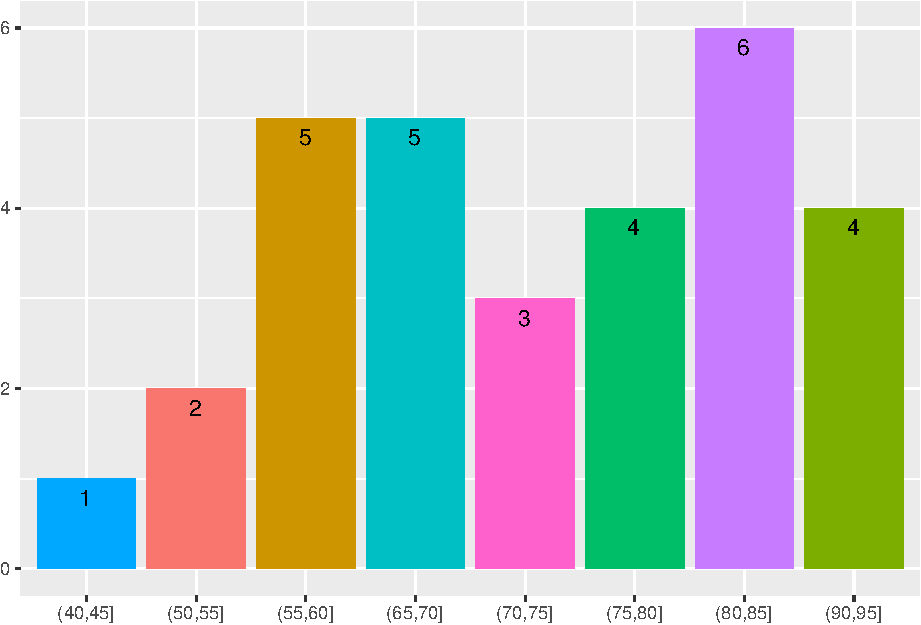
\includegraphics{ita_files/figure-latex/unnamed-chunk-9-1.pdf}

\subsection{学生成绩}

\begin{longtable}{c|c|c|c}
\hline
id & name & grade & zscore\\
\hline
2016052128 & 王睿 & 94 & 1.44396334\\
\hline
2016052104 & 康倍瑄 & 89 & 1.12809636\\
\hline
2016052118 & 陈雪婷 & 89 & 1.12809636\\
\hline
2016052124 & 常展赫 & 89 & 1.12809636\\
\hline
2016052123 & 吴承蔚 & 88 & 1.06492297\\
\hline
2016052117 & 王星悦 & 87 & 1.00174957\\
\hline
2016052129 & 吴鸿丽 & 83 & 0.74905598\\
\hline
2016052102 & 翟思楠 & 82 & 0.68588259\\
\hline
2016052106 & 孔永强 & 81 & 0.62270919\\
\hline
2016052127 & 孙思哲 & 78 & 0.43318900\\
\hline
2016052112 & 陈浩 & 77 & 0.37001561\\
\hline
2016052122 & 郭欣 & 77 & 0.37001561\\
\hline
2016052107 & 徐孟 & 76 & 0.30684221\\
\hline
2016052105 & 黄刚 & 75 & 0.24366881\\
\hline
2016052113 & 张云柱 & 72 & 0.05414863\\
\hline
2016052111 & 杨富丞 & 69 & -0.13537156\\
\hline
2016052115 & 多晶蕾 & 69 & -0.13537156\\
\hline
2016052126 & 陈宏瑞 & 69 & -0.13537156\\
\hline
2016052103 & 樊绪仝 & 67 & -0.26171836\\
\hline
2016052101 & 惠千益 & 66 & -0.32489175\\
\hline
2016052125 & 赵孟羽 & 64 & -0.45123854\\
\hline
2016052120 & 荣凌波 & 62 & -0.57758534\\
\hline
2016052119 & 李欣 & 60 & -0.70393213\\
\hline
2016052130 & 汤敏丹 & 57 & -0.89345232\\
\hline
2016052110 & 王晟欣 & 54 & -1.08297251\\
\hline
2016052114 & 陈玉欣 & 54 & -1.08297251\\
\hline
2016052116 & 张湘漪 & 38 & -2.09374685\\
\hline
2016052108 & 龙鑫 & 26 & -2.85182760\\
\hline
\end{longtable}

\section{试题质量分析}

\subsection{难度与区分度趋势图}

\subsubsection{整卷趋势}

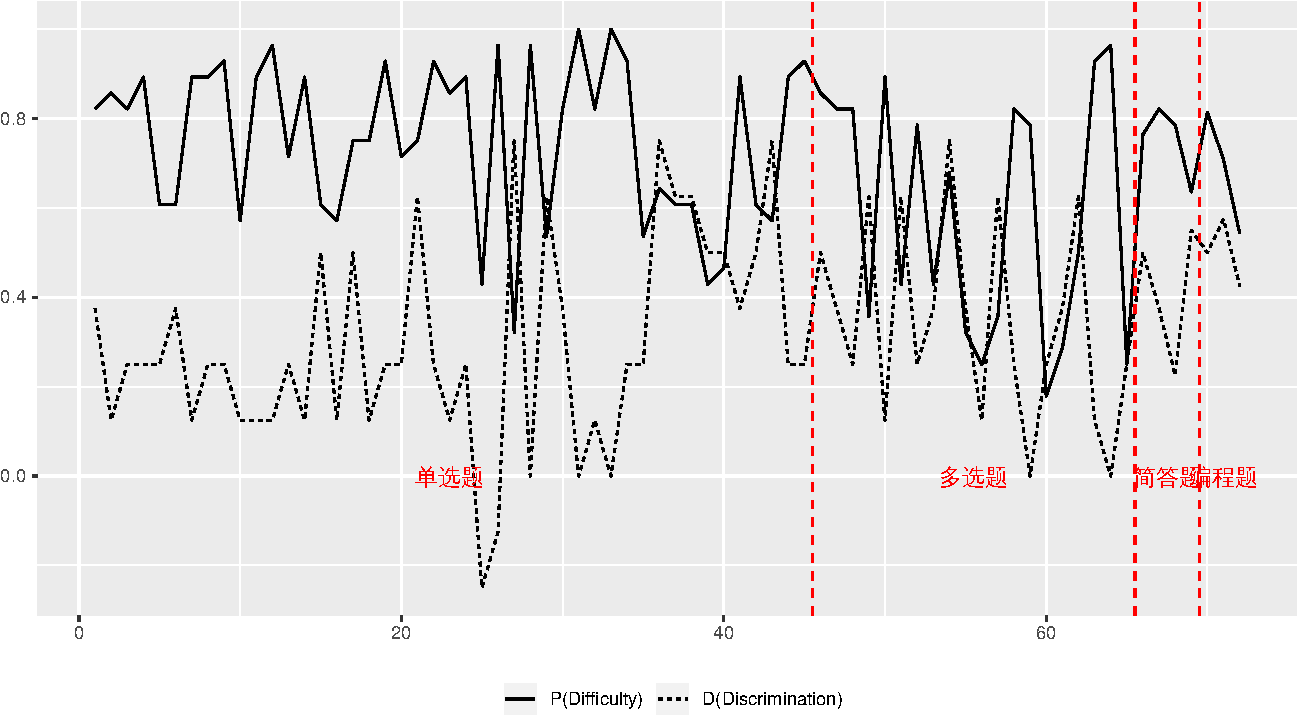
\includegraphics{ita_files/figure-latex/unnamed-chunk-14-1.pdf}

\subsubsection{题型趋势}

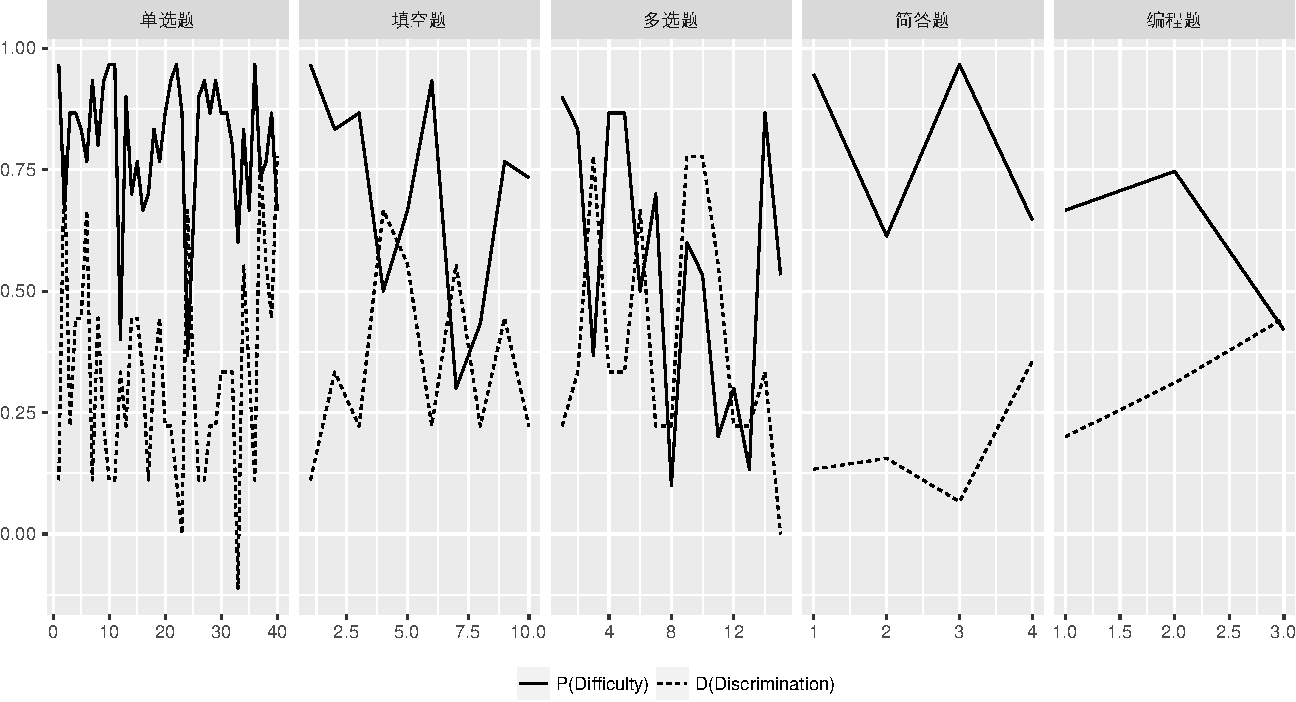
\includegraphics{ita_files/figure-latex/unnamed-chunk-16-1.pdf}

\subsubsection{章节趋势}

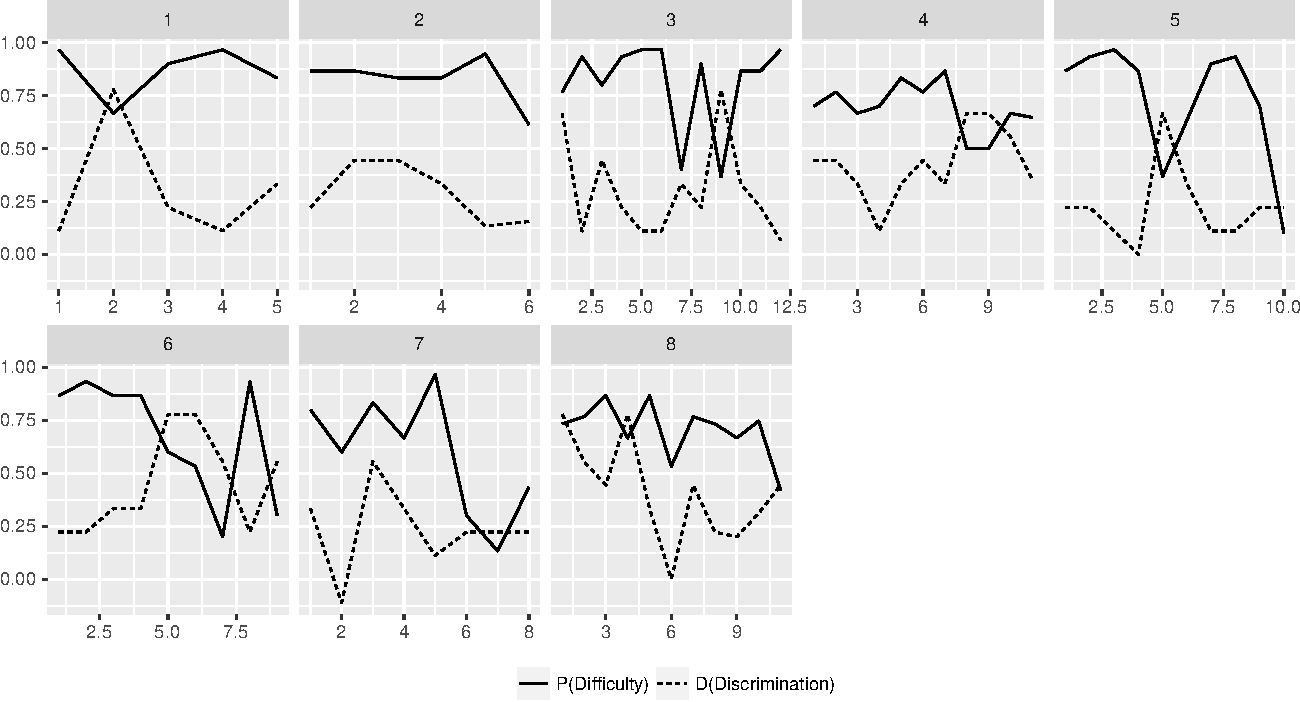
\includegraphics{ita_files/figure-latex/unnamed-chunk-18-1.pdf}

\subsection{难度与区分度分布图}

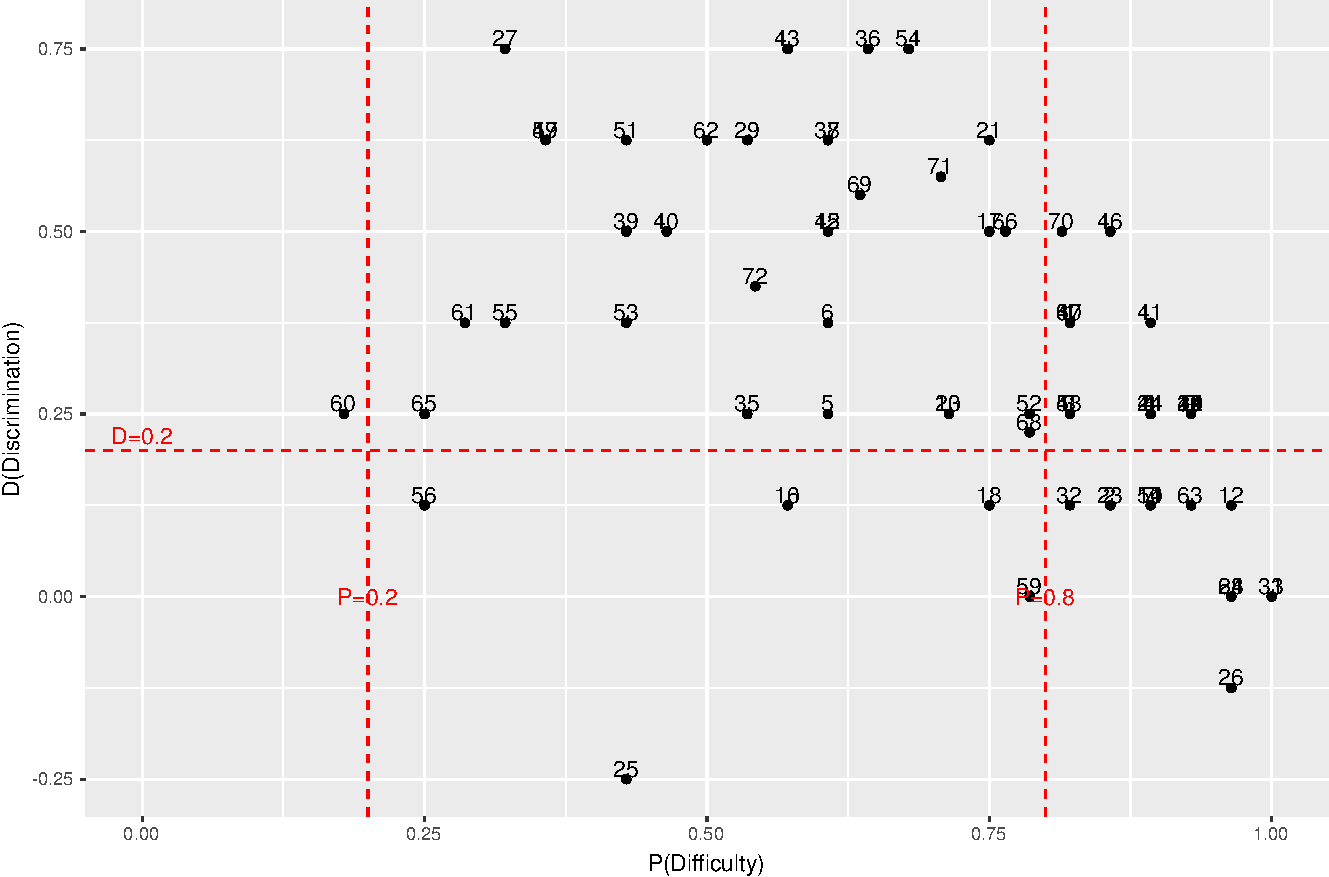
\includegraphics{ita_files/figure-latex/unnamed-chunk-20-1.pdf}

\subsection{有待改进的题目}

部分题目(16/72)有待改进:难度不适宜(P\textgreater{}=0.80或者P\textless{}=0.20)且区分度不好(0\textless{}D\textless{}=0.20),或者没有区分度(D\textless{}=0)。

\begin{longtable}{c|c|c|c|c|c|c|c}
\hline
id & type & chapter & mark & mean & sd & P & D\\
\hline
2 & 单选题 & 1 & 1 & 0.857 & 0.356 & 0.857 & 0.125\\
\hline
7 & 单选题 & 3 & 1 & 0.893 & 0.315 & 0.893 & 0.125\\
\hline
11 & 单选题 & 3 & 1 & 0.893 & 0.315 & 0.893 & 0.125\\
\hline
12 & 单选题 & 4 & 1 & 0.964 & 0.189 & 0.964 & 0.125\\
\hline
14 & 单选题 & 4 & 1 & 0.893 & 0.315 & 0.893 & 0.125\\
\hline
23 & 单选题 & 5 & 1 & 0.857 & 0.356 & 0.857 & 0.125\\
\hline
25 & 单选题 & 5 & 1 & 0.429 & 0.504 & 0.429 & -0.250\\
\hline
26 & 单选题 & 5 & 1 & 0.964 & 0.189 & 0.964 & -0.125\\
\hline
28 & 单选题 & 5 & 1 & 0.964 & 0.189 & 0.964 & 0.000\\
\hline
31 & 单选题 & 6 & 1 & 1.000 & 0.000 & 1.000 & 0.000\\
\hline
32 & 单选题 & 6 & 1 & 0.821 & 0.390 & 0.821 & 0.125\\
\hline
33 & 单选题 & 7 & 1 & 1.000 & 0.000 & 1.000 & 0.000\\
\hline
50 & 多选题 & 3 & 1 & 0.893 & 0.315 & 0.893 & 0.125\\
\hline
59 & 多选题 & 7 & 1 & 0.786 & 0.418 & 0.786 & 0.000\\
\hline
63 & 多选题 & 8 & 1 & 0.929 & 0.262 & 0.929 & 0.125\\
\hline
64 & 多选题 & 8 & 1 & 0.964 & 0.189 & 0.964 & 0.000\\
\hline
\end{longtable}

\section{题型章节分析}

\subsection{题型分析}

\begin{longtable}{c|c|c|c|c|c|c|c}
\hline
type & number & score & percent & mean & sd & P & D\\
\hline
单选题 & 45 & 45 & 0.45 & 34.071 & 0.180 & 0.757 & 0.292\\
\hline
多选题 & 20 & 20 & 0.20 & 11.714 & 0.271 & 0.586 & 0.344\\
\hline
简答题 & 4 & 20 & 0.20 & 15.036 & 0.404 & 0.752 & 0.412\\
\hline
编程题 & 3 & 15 & 0.15 & 10.321 & 0.684 & 0.688 & 0.500\\
\hline
\end{longtable}

\subsection{章节分析}

\begin{longtable}{c|c|c|c|c|c|c|c}
\hline
chapter & number & score & percent & mean & sd & P & D\\
\hline
1 & 4 & 4 & 0.04 & 3.357 & 0.021 & 0.839 & 0.344\\
\hline
2 & 4 & 8 & 0.08 & 6.143 & 1.529 & 0.768 & 0.406\\
\hline
3 & 12 & 20 & 0.20 & 15.321 & 1.296 & 0.766 & 0.294\\
\hline
4 & 10 & 10 & 0.10 & 7.393 & 0.168 & 0.739 & 0.262\\
\hline
5 & 14 & 18 & 0.18 & 11.786 & 0.718 & 0.655 & 0.361\\
\hline
6 & 5 & 5 & 0.05 & 3.821 & 0.240 & 0.764 & 0.275\\
\hline
7 & 12 & 12 & 0.12 & 6.964 & 0.241 & 0.580 & 0.396\\
\hline
8 & 11 & 23 & 0.23 & 16.357 & 1.309 & 0.711 & 0.435\\
\hline
\end{longtable}

\section{选择题分析}

\subsection{单选题分析}

\begin{longtable}{c|c|c|c|c|c|c|c|c}
\hline
id & answer & mark & mean & sd & P & D & RPB & IRI\\
\hline
1 & D & 1 & 0.821 & 0.390 & 0.821 & 0.375 & 0.376 & 0.144\\
\hline
2 & B & 1 & 0.857 & 0.356 & 0.857 & 0.125 & 0.010 & 0.004\\
\hline
3 & B & 1 & 0.821 & 0.390 & 0.821 & 0.250 & 0.214 & 0.082\\
\hline
4 & B & 1 & 0.893 & 0.315 & 0.893 & 0.250 & 0.412 & 0.127\\
\hline
5 & B & 1 & 0.607 & 0.497 & 0.607 & 0.250 & 0.163 & 0.079\\
\hline
6 & A & 1 & 0.607 & 0.497 & 0.607 & 0.375 & 0.257 & 0.125\\
\hline
7 & B & 1 & 0.893 & 0.315 & 0.893 & 0.125 & 0.018 & 0.006\\
\hline
8 & D & 1 & 0.893 & 0.315 & 0.893 & 0.250 & 0.612 & 0.189\\
\hline
9 & D & 1 & 0.929 & 0.262 & 0.929 & 0.250 & 0.484 & 0.125\\
\hline
10 & B & 1 & 0.571 & 0.504 & 0.571 & 0.125 & 0.143 & 0.071\\
\hline
11 & D & 1 & 0.893 & 0.315 & 0.893 & 0.125 & 0.293 & 0.091\\
\hline
12 & B & 1 & 0.964 & 0.189 & 0.964 & 0.125 & 0.138 & 0.026\\
\hline
13 & C & 1 & 0.714 & 0.460 & 0.714 & 0.250 & 0.341 & 0.154\\
\hline
14 & B & 1 & 0.893 & 0.315 & 0.893 & 0.125 & 0.278 & 0.086\\
\hline
15 & A & 1 & 0.607 & 0.497 & 0.607 & 0.500 & 0.384 & 0.187\\
\hline
16 & A & 1 & 0.571 & 0.504 & 0.571 & 0.125 & 0.217 & 0.107\\
\hline
17 & A & 1 & 0.750 & 0.441 & 0.750 & 0.500 & 0.435 & 0.188\\
\hline
18 & B & 1 & 0.750 & 0.441 & 0.750 & 0.125 & 0.334 & 0.145\\
\hline
19 & D & 1 & 0.929 & 0.262 & 0.929 & 0.250 & 0.484 & 0.125\\
\hline
20 & B & 1 & 0.714 & 0.460 & 0.714 & 0.250 & 0.021 & 0.010\\
\hline
21 & A & 1 & 0.750 & 0.441 & 0.750 & 0.625 & 0.610 & 0.264\\
\hline
22 & B & 1 & 0.929 & 0.262 & 0.929 & 0.250 & 0.466 & 0.120\\
\hline
23 & B & 1 & 0.857 & 0.356 & 0.857 & 0.125 & 0.017 & 0.006\\
\hline
24 & D & 1 & 0.893 & 0.315 & 0.893 & 0.250 & 0.419 & 0.130\\
\hline
25 & B & 1 & 0.429 & 0.504 & 0.429 & -0.250 & -0.040 & -0.020\\
\hline
26 & B & 1 & 0.964 & 0.189 & 0.964 & -0.125 & -0.221 & -0.041\\
\hline
27 & A & 1 & 0.321 & 0.476 & 0.321 & 0.750 & 0.549 & 0.257\\
\hline
28 & C & 1 & 0.964 & 0.189 & 0.964 & 0.000 & -0.072 & -0.013\\
\hline
29 & C & 1 & 0.536 & 0.508 & 0.536 & 0.625 & 0.400 & 0.199\\
\hline
30 & B & 1 & 0.821 & 0.390 & 0.821 & 0.375 & 0.226 & 0.087\\
\hline
31 & C & 1 & 1.000 & 0.000 & 1.000 & 0.000 & NA & NA\\
\hline
32 & B & 1 & 0.821 & 0.390 & 0.821 & 0.125 & 0.178 & 0.068\\
\hline
33 & D & 1 & 1.000 & 0.000 & 1.000 & 0.000 & NA & NA\\
\hline
34 & C & 1 & 0.929 & 0.262 & 0.929 & 0.250 & 0.698 & 0.180\\
\hline
35 & C & 1 & 0.536 & 0.508 & 0.536 & 0.250 & 0.363 & 0.181\\
\hline
36 & C & 1 & 0.643 & 0.488 & 0.643 & 0.750 & 0.525 & 0.251\\
\hline
37 & D & 1 & 0.607 & 0.497 & 0.607 & 0.625 & 0.402 & 0.197\\
\hline
38 & A & 1 & 0.607 & 0.497 & 0.607 & 0.625 & 0.534 & 0.261\\
\hline
39 & A & 1 & 0.429 & 0.504 & 0.429 & 0.500 & 0.266 & 0.132\\
\hline
40 & A & 1 & 0.464 & 0.508 & 0.464 & 0.500 & 0.332 & 0.166\\
\hline
41 & B & 1 & 0.893 & 0.315 & 0.893 & 0.375 & 0.686 & 0.212\\
\hline
42 & B & 1 & 0.607 & 0.497 & 0.607 & 0.500 & 0.464 & 0.226\\
\hline
43 & B & 1 & 0.571 & 0.504 & 0.571 & 0.750 & 0.611 & 0.303\\
\hline
44 & A & 1 & 0.893 & 0.315 & 0.893 & 0.250 & 0.389 & 0.120\\
\hline
45 & C & 1 & 0.929 & 0.262 & 0.929 & 0.250 & 0.555 & 0.143\\
\hline
\end{longtable}

\begin{itemize}
\tightlist
\item
  RPB:点双列相关系数。
\item
  IRI:试题的信度。
\end{itemize}

\subsection{多选题分析}

\begin{longtable}{c|c|c|c|c|c|c|c|c}
\hline
id & answer & mark & mean & sd & P & D & RPB & IRI\\
\hline
46 & ABCD & 1 & 0.857 & 0.356 & 0.857 & 0.500 & 0.679 & 0.238\\
\hline
47 & ABCD & 1 & 0.821 & 0.390 & 0.821 & 0.375 & 0.538 & 0.206\\
\hline
48 & ABCD & 1 & 0.821 & 0.390 & 0.821 & 0.250 & 0.454 & 0.174\\
\hline
49 & AC & 1 & 0.357 & 0.488 & 0.357 & 0.625 & 0.458 & 0.219\\
\hline
50 & ABCD & 1 & 0.893 & 0.315 & 0.893 & 0.125 & 0.293 & 0.091\\
\hline
51 & ABCD & 1 & 0.429 & 0.504 & 0.429 & 0.625 & 0.484 & 0.239\\
\hline
52 & AB & 1 & 0.786 & 0.418 & 0.786 & 0.250 & 0.436 & 0.179\\
\hline
53 & AB & 1 & 0.429 & 0.504 & 0.429 & 0.375 & 0.275 & 0.136\\
\hline
54 & ABCD & 1 & 0.679 & 0.476 & 0.679 & 0.750 & 0.645 & 0.301\\
\hline
55 & ABC & 1 & 0.321 & 0.476 & 0.321 & 0.375 & 0.200 & 0.093\\
\hline
56 & AB & 1 & 0.250 & 0.441 & 0.250 & 0.125 & -0.032 & -0.014\\
\hline
57 & BCD & 1 & 0.357 & 0.488 & 0.357 & 0.625 & 0.472 & 0.226\\
\hline
58 & ABCD & 1 & 0.821 & 0.390 & 0.821 & 0.250 & 0.340 & 0.130\\
\hline
59 & AB & 1 & 0.786 & 0.418 & 0.786 & 0.000 & 0.105 & 0.043\\
\hline
60 & ABCD & 1 & 0.179 & 0.390 & 0.179 & 0.250 & 0.241 & 0.092\\
\hline
61 & AD & 1 & 0.286 & 0.460 & 0.286 & 0.375 & 0.401 & 0.181\\
\hline
62 & ABC & 1 & 0.500 & 0.509 & 0.500 & 0.625 & 0.445 & 0.223\\
\hline
63 & ABC & 1 & 0.929 & 0.262 & 0.929 & 0.125 & 0.190 & 0.049\\
\hline
64 & AB & 1 & 0.964 & 0.189 & 0.964 & 0.000 & 0.064 & 0.012\\
\hline
65 & ABC & 1 & 0.250 & 0.441 & 0.250 & 0.250 & 0.111 & 0.048\\
\hline
\end{longtable}

\begin{itemize}
\tightlist
\item
  RPB:点双列相关系数。
\item
  IRI:试题的信度。
\end{itemize}

\end{document}
